%=================================================================
% Post-Conflict LULC Transitions in Magdalena Medio
% Format: elsarticle class, natbib (Applied Geography submission)
%=================================================================
\documentclass[preprint,12pt]{elsarticle}

% Math
\usepackage{amsmath}
\usepackage{amsfonts}

% Graphics
\usepackage{graphicx}
\graphicspath{{./figures/}}

% Tables
\usepackage{booktabs}
\usepackage{multirow}
\usepackage{threeparttable}

% Units
\usepackage{siunitx}
\sisetup{group-separator={,}, group-minimum-digits=4, separate-uncertainty=true}

% Fonts and encoding
\usepackage[utf8]{inputenc}
\usepackage[T1]{fontenc}
\DeclareUnicodeCharacter{0301}{\'{}}
\usepackage{csquotes}

% Hyperlinks
\usepackage[colorlinks=true, allcolors=blue]{hyperref}
\usepackage{url}

% Lists
\usepackage{enumitem}

% Floats
\usepackage{float}

% Line numbering (uncomment for review)
\usepackage{lineno}
\linenumbers

% Journal target
\journal{Applied Geography}
\biboptions{authoryear}

% Suppress PDF warnings
\pdfsuppresswarningpagegroup=1


\begin{document}

\begin{frontmatter}

\title{Accelerating Deforestation After Peace: Land Use Transitions and Carbon Loss in Colombia's Magdalena Medio (2012--2024)}

\author[eafit1]{Cristian Espinal Maya\corref{cor1}}
\ead{cjespinalm@eafit.edu.co}
\cortext[cor1]{Corresponding author}

\author[eafit2]{Santiago Jim\'{e}nez Londo\~{n}o}
\ead{sjimene8@eafit.edu.co}

\address[eafit1]{School of Finance, Economics and Government, Universidad EAFIT, Medell\'{i}n 050022, Colombia}
\address[eafit2]{School of Applied Sciences and Engineering, Universidad EAFIT, Medell\'{i}n 050022, Colombia}

\begin{abstract}
Armed conflict has historically shaped land use patterns in tropical landscapes, yet environmental dynamics accompanying post-agreement transitions remain poorly understood. This study analyzes land use and land cover change (LULCC) in Colombia's Magdalena Medio region across four periods spanning the pre-peace agreement era through post-agreement implementation (2012--2024). Using Random Forest classification in Google Earth Engine with Landsat~8/9 and Sentinel-2 imagery, we produced four LULC maps (2013, 2016, 2020, 2024) assessed through \citet{Olofsson2014} stratified area estimators with 95\% confidence intervals (adjusted overall accuracies: 59--63\%). Cross-validation against four independent products (MapBiomas, ESA WorldCover, Dynamic World, MODIS Land Cover) confirmed directional consistency in forest decline. Estimated total forest cover (dense~$+$~secondary) declined from ${\sim}$2,021,000~ha (2013) to ${\sim}$1,591,000~ha (2024), a net loss of ${\sim}$21\% ($\pm$18\%), with forest-to-pasture conversion as the dominant transition. Carbon stocks (IPCC Tier~2) declined from $435 \pm 76$ to $374 \pm 74$~Tg~C, with Monte Carlo simulation (10,000 correlated draws) yielding P(net loss)~$= 0.953$. Getis-Ord Gi* identified 648 deforestation hotspot cells (99\% confidence) concentrated along river corridors. Geographically Weighted Regression confirmed spatially varying driver effects. These findings document accelerated post-agreement deforestation and provide inputs for territorial planning, contributing to SDGs~6, 13, 15, and~16.
\end{abstract}

\begin{keyword}
Land use/land cover change \sep Post-conflict deforestation \sep Ecosystem services \sep Google Earth Engine \sep Magdalena Medio \sep Carbon storage \sep Remote sensing
\end{keyword}

\end{frontmatter}


%%%%%%%%%%%%%%%%%%%%%%%%%%%%%%%%%%%%%%%%%%
\section{Introduction}
%%%%%%%%%%%%%%%%%%%%%%%%%%%%%%%%%%%%%%%%%%

\subsection{Armed Conflict, Land Systems, and Tropical Deforestation}

Land system science provides a framework for understanding the coupled human--environment interactions that drive land use transitions in complex socio-ecological contexts \citep{Verburg2015,Turner2007}. Within this framework, armed conflict constitutes a potent but paradoxical driver of tropical land system change. While active warfare often restricts access to remote areas---creating inadvertent ``gunpoint conservation'' \citep{Alvarez2003}---the cessation of hostilities can trigger rapid deforestation as governance vacuums emerge and previously inaccessible territories become open to agricultural expansion, land speculation, and resource extraction \citep{Prem2020,Clerici2020}. This paradox has been documented across multiple post-conflict contexts, from Sierra Leone to Nepal \citep{Landholm2019Diverging}, but nowhere has it been as acutely manifest as in Colombia \citep{Fagan2020,CastroNunez2022,MurilloSandoval2021}.

Colombia's 2016 peace agreement with the FARC-EP guerrilla ended over five decades of internal armed conflict. The environmental consequences were swift: deforestation rates increased by 44\% nationally between 2015 and 2017, with the most pronounced increases in former FARC-controlled territories \citep{IDEAM2018,Prem2020}. \citet{Clerici2020} documented a 177\% increase in deforestation rates within and around protected areas in post-conflict zones. \citet{MurilloSandoval2023Post} identified coca cultivation and cattle ranching as interacting drivers of post-agreement landscape change, while \citet{VanegasCubillos2022Forest} provided a systematic review linking forest-policy dynamics to the post-conflict transition. \citet{Cantillo2022Armed} demonstrated spatiotemporal associations between deforestation and armed conflict intensity during 2000--2018, and \citet{Davalos2021Forests} analyzed the coca-forest-pasture dynamics that underpin deforestation in former conflict zones. \citet{CastroNunez2022} identified extensive cattle ranching and land speculation---rather than smallholder agriculture---as the primary drivers of forest conversion \citep[see also][]{Pacheco2009,Negret2019}. \citet{Sierra2017} emphasized the urgent need for ecological monitoring systems during Colombia's rapid post-agreement transition.

Despite this growing body of evidence, three critical gaps persist. First, most studies rely on the Hansen Global Forest Change dataset \citep{Hansen2013}, which captures only binary forest loss/gain rather than complete multi-class land use transitions---yet understanding \textit{what replaces forest} is essential for estimating ecosystem service impacts. Second, the existing literature overwhelmingly focuses on the Amazon and Pacific regions \citep{Prem2020,Clerici2020,MurilloSandoval2021,MurilloSandoval2023Disentangling,Negret2019}, leaving other conflict-affected landscapes inadequately studied. Third, few studies integrate land cover classification with ecosystem service quantification and spatial driver analysis within a unified analytical framework, limiting the capacity for comprehensive territorial planning in post-agreement contexts.

\subsection{The Magdalena Medio: A Critical Knowledge Gap}

The Magdalena Medio region, situated in the middle valley of the Magdalena River between the Central and Eastern Cordilleras, represents a critical yet remarkably understudied landscape in the context of post-agreement environmental change. Spanning approximately 36,800~km$^2$ across 30 municipalities in the departments of Santander, Antioquia, Bol\'{i}var, and Cesar, this region was identified as a deforestation hotspot by \citet{SanchezCuervo2013}, who notably highlighted the near-complete absence of protected areas. \citet{Hoffmann2018Local} documented local deforestation drivers in comparable Andean-Amazonian foothills, but no comprehensive multi-class LULCC study exists for the Magdalena Medio post-2016.

The region's biophysical characteristics---lowland tropical humid forest (50--500~m~a.s.l.), mean annual precipitation of 2,700--3,000~mm, and fertile alluvial soils---make it both ecologically valuable and economically attractive for agricultural conversion. Its economy combines petroleum extraction (centered on Barrancabermeja), extensive cattle ranching, oil palm cultivation, artisanal gold mining, and illicit coca cultivation---a suite of pressures representative of the complex socio-environmental dynamics characterizing post-agreement tropical landscapes. Most municipalities in the study area are designated as PDET territories (Planes de Desarrollo con Enfoque Territorial), prioritized for post-conflict territorial development, making it a natural laboratory for studying the interplay between peacebuilding governance and land system change.

This study addresses this knowledge gap through the first comprehensive multi-temporal, multi-class LULCC analysis of the Magdalena Medio (2012--2024), integrating land cover classification with ecosystem service quantification and spatial driver analysis using Google Earth Engine \citep{Gorelick2017}. We employ Random Forest classification \citep{Breiman2001} with Landsat~8/9 and Sentinel-2 imagery \citep{Wulder2022,Drusch2012}, \citet{Olofsson2014} stratified area estimators for unbiased area estimation, IPCC Tier~2 carbon pools \citep{IPCC2006,Alvarez2012}, spatial autocorrelation and hotspot analysis \citep{Moran1950,Getis1992,Anselin1995}, Geographically Weighted Regression \citep{Fotheringham2002} for spatially varying driver analysis, and multi-product cross-validation to ensure robustness of findings.

\subsection{Research Objectives and Hypotheses}

This study aims to analyze the spatiotemporal dynamics of LULCC in Colombia's Magdalena Medio region during 2012--2024, quantifying their impact on ecosystem services and evaluating spatial patterns of change associated with the post-peace agreement transition. Specifically, we address four objectives:

\begin{description}
\item[RO1.] Classify and map LULC for four periods (2013, 2016, 2020, 2024) using Random Forest in GEE, and generate transition matrices characterizing pre- and post-agreement change trajectories.
\item[RO2.] Identify spatial patterns and hotspots of LULCC through spatial autocorrelation analysis (Moran's~$I$), hotspot detection (Getis-Ord Gi*), and deforestation intensity mapping.
\item[RO3.] Quantify ecosystem service changes (carbon storage, water yield, habitat quality) associated with LULCC using IPCC Tier~2 carbon pools and proxy models integrated with GEE.
\item[RO4.] Analyze the socio-environmental drivers of deforestation through GWR and project future LULC scenarios for 2030 and 2040 under three pathways (business-as-usual, conservation, and PDET implementation).
\end{description}

We test four hypotheses:

\textbf{H1.} The rate of forest-to-pasture conversion increased significantly in the post-agreement period (2017--2024) relative to the pre-agreement period (2012--2016), temporally associated with cattle ranching expansion and land speculation in areas of former FARC presence.

\textbf{H2.} Post-agreement LULCC exhibits significant spatial clustering (Moran's~$I > 0$), with deforestation hotspots concentrated in areas of low institutional presence and high accessibility.

\textbf{H3.} Post-agreement deforestation has generated a significant loss ($>$10\%) in regional carbon stocks, reduced hydrological regulation, and decreased habitat quality.

\textbf{H4.} Deforestation drivers exhibit significant spatial heterogeneity, with GWR substantially outperforming global OLS regression and revealing spatially varying driver effects.


%%%%%%%%%%%%%%%%%%%%%%%%%%%%%%%%%%%%%%%%%%
\section{Study Area}
%%%%%%%%%%%%%%%%%%%%%%%%%%%%%%%%%%%%%%%%%%

\subsection{Geographic Setting}

The Magdalena Medio region is located in the middle valley of the Magdalena River, Colombia's principal waterway \citep{Restrepo2006}, between 6.0$^\circ$N--8.0$^\circ$N latitude and 73.5$^\circ$W--75.0$^\circ$W longitude (Figure~\ref{fig:study_area}). The study area encompasses 30 municipalities across four departments: Santander (14 municipalities, including the regional capital Barrancabermeja), Antioquia (6 municipalities), Bol\'{i}var (6 municipalities), and Cesar (4 municipalities), covering approximately 36,800~km$^2$.

The landscape is characterized by lowland terrain (predominantly 50--200~m~a.s.l.) within the humid tropical forest life zone \citep{Holdridge1967}. Mean annual temperature ranges from 27.0 to 28.7$^\circ$C (based on MODIS LST 2012--2024), with annual precipitation averaging 2,852~mm (CHIRPS 2012--2024; range 2,597--3,464~mm) following a bimodal regime with peaks in April--May and September--November. Soils are predominantly alluvial with high agricultural potential in the river floodplain, transitioning to lateritic and hillslope soils in the piedmont areas.

\begin{figure}[!ht]
\centering
\includegraphics[width=\textwidth]{fig01_study_area_choropleth.png}
\caption{Study area: (a)~Location of the Magdalena Medio in Colombia; (b)~Veredal-level choropleth of dominant LULC class (2024) with municipal boundaries (thin gray lines) and departmental boundaries (thick black lines). The study area encompasses 30 municipalities (${\sim}$36,817~km$^2$) across four departments (Santander, Antioquia, Bol\'{i}var, Cesar).\label{fig:study_area}}
\end{figure}

\subsection{Socioeconomic and Conflict Context}

The Magdalena Medio has been historically one of Colombia's most conflict-affected regions, with overlapping presence of FARC-EP, ELN, and paramilitary groups throughout the late 20th and early 21st centuries. The region's strategic importance---controlling riverine transport along the Magdalena and hosting Colombia's largest oil refinery in Barrancabermeja---made it a focal point of armed contestation.

The 2016 peace agreement designated most municipalities in the study area as PDET territories, prioritized for post-conflict territorial development. However, the transition has been marked by governance vacuums, the emergence of dissident armed groups, and accelerated natural resource extraction \citep{Fagan2020}. The region's economy combines formal industries (petroleum, oil palm) with extensive cattle ranching, artisanal mining, and coca cultivation, creating a complex mosaic of land use pressures.

\subsection{Analysis Periods}

We defined four analysis periods aligned with key political milestones:

\begin{itemize}
\item \textbf{T1: Pre-agreement (2012--2014):} Active conflict with ongoing Havana peace negotiations; FARC territorial control restricts access to forested areas. Representative year: 2013.
\item \textbf{T2: Transition (2015--2017):} Ceasefire, agreement signing (November 2016), and initial FARC demobilization; governance vacuums emerge. Representative year: 2016.
\item \textbf{T3: Early post-agreement (2019--2021):} PDET implementation begins; COVID-19 pandemic; cattle ranching expansion accelerates. Representative year: 2020.
\item \textbf{T4: Recent post-agreement (2023--2024):} Petro government's ``Total Peace'' policy; national deforestation reduction efforts; continued PDET implementation. Representative year: 2024.
\end{itemize}


%%%%%%%%%%%%%%%%%%%%%%%%%%%%%%%%%%%%%%%%%%
\section{Materials and Methods}
%%%%%%%%%%%%%%%%%%%%%%%%%%%%%%%%%%%%%%%%%%

\subsection{Data Sources}

\subsubsection{Satellite Imagery}

Multi-temporal composites were generated from Landsat~8/9 Collection~2 Level~2 Surface Reflectance (USGS; 30~m; \citealp{Wulder2022}) and Sentinel-2 SR Harmonized (ESA/Copernicus; 10--20~m; \citealp{Drusch2012}) imagery accessed through Google Earth Engine (GEE project: ee-maestria-tesis). For T1~(2013), only Landsat~8 was available (157 images). For T2--T3, harmonized Landsat~8+Sentinel-2 composites were produced using common band nomenclature, yielding 210~(T2) and 1191~(T3) images. For T4~(2024), only Landsat~8/9 was used (355 images). Cloud masking followed sensor-specific protocols: QA\_PIXEL bitwise flags for Landsat and Scene Classification Layer bands for Sentinel-2. Details of sensor parameters, scaling factors, and cloud masking protocols are provided in Tables~S2--S4 (Supplementary Materials).

\subsubsection{Ancillary Datasets}

Topographic variables (elevation, slope) were derived from SRTM 30~m. Precipitation data were obtained from CHIRPS Daily v2.0 \citep{Funk2015}. Land surface temperature (LST) came from MODIS MOD11A2 v061. Population density was sourced from WorldPop (100~m), settlement patterns from GHSL SMOD 2020 (1~km), and permanent water extent from JRC Global Surface Water v1.4 (30~m). Hansen Global Forest Change v1.12 \citep{Hansen2013} provided independent forest loss validation and reference data for training sample generation. For water yield estimation, TerraClimate \citep{Abatzoglou2018} provided monthly actual evapotranspiration (AET) and potential evapotranspiration (PET) at ${\sim}$4~km resolution, cross-validated against ERA5-Land monthly aggregates.

\subsection{LULC Classification}

\subsubsection{Classification Scheme}

We adopted a seven-class LULC scheme based on dominant land covers in the Magdalena Medio: (1)~Dense forest (canopy cover $>$60\%), (2)~Secondary/fragmented forest (canopy cover 30--60\%, successional), (3)~Pastures/grasslands, (4)~Croplands (oil palm, rice, coca, other), (5)~Water bodies (rivers, wetlands, reservoirs), (6)~Urban/built-up, and (7)~Bare soil/mining.

\subsubsection{Training Sample Generation}

Reference LULC data were generated through a rule-based approach combining: (i)~Hansen GFC v1.12 treecover2000 and loss year for forest/non-forest discrimination, (ii)~JRC Global Surface Water for permanent water bodies (occurrence $>$ 80\%), (iii)~GHSL SMOD for urban centres (smod\_code $\geq$ 30), and (iv)~proximity to cropland indicators for agricultural areas. Stratified random sampling generated approximately 300 points per class (total ${\sim}$1000--1100 per period), split 70/30 for training and validation. While seven classes were defined, Croplands (class~4) and Bare soil (class~7) had zero mapped area in all periods; the effective classification therefore operates on five active classes. The absence of mapped croplands reflects spectral similarity between oil palm canopy and forest/pasture classes in annual median composites at 30~m resolution. Consequently, the ``Pastures'' class should be interpreted as a composite category encompassing non-forest, non-urban, non-water vegetated and open land, including cattle pastures, oil palm, smallholder crops, and disturbed areas.

\subsubsection{Feature Extraction and Classification}

For each period, pixel-level composites included 12 features: 6 surface reflectance bands (blue, green, red, NIR, SWIR1, SWIR2), 4 spectral indices (NDVI, NDWI, NDBI, NBR), and 2 topographic variables (elevation, slope). Classification used Random Forest \citep[\texttt{ee.Classifier.smileRandomForest};][]{Breiman2001} with 200 trees, minimum leaf population of~5, and bag fraction of 0.632. Post-processing enforced water bodies using JRC Global Surface Water pixels with $>$80\% temporal occurrence.

\subsection{Accuracy Assessment and Multi-Product Validation}

Classification accuracy was evaluated using error matrices from the 30\% hold-out validation set \citep{Congalton1991,Foody2002}. Following \citet{Olofsson2014} and \citet{Stehman2019}, we applied stratified area estimators that weight confusion matrix entries by mapped-class proportions to obtain unbiased area estimates with 95\% confidence intervals. Two zero-area classes were dropped, yielding an effective 5-class system. The Kappa coefficient was replaced by quantity disagreement~(QD) and allocation disagreement~(AD) following \citet{Pontius2011} and \citet{Foody2020}.

To assess the robustness of forest change findings despite moderate per-pixel accuracy, we cross-validated forest area trends against four independent products: MapBiomas Colombia Collection~1, ESA WorldCover v200 (10~m, 2021), Google Dynamic World v1 (10~m, 2015--2024), and MODIS MCD12Q1 v061 (500~m, 2013--2023). For each product, forest-equivalent classes were identified and total forest area within the study boundary was computed. Directional agreement (decline/stable/increase) was evaluated for each inter-period interval.

\subsection{Change Detection}

Three transition matrices were computed for sequential period pairs (T1$\rightarrow$T2, T2$\rightarrow$T3, T3$\rightarrow$T4). Areas (ha) for each from-to class combination were calculated via pixel counting, yielding persistence, gross gains, gross losses, net change, and annual rates for each class \citep{Puyravaud2003}. Forest loss was cross-validated against Hansen GFC v1.12 loss year data, aggregated by analysis period.

\subsection{Spatial Statistical Analysis}

\subsubsection{Spatial Autocorrelation and Hotspot Analysis}

Moran's~$I$ global statistic \citep{Moran1950,Anselin1995} was computed to test for spatial autocorrelation in deforestation rates across 1$\times$1~km grid cells, using distance-based Queen contiguity weights. Getis-Ord Gi* local statistics \citep{Getis1992} identified statistically significant hotspots and coldspots at 90\%, 95\%, and 99\% confidence levels. Local Moran's~$I$ (LISA) cluster analysis classified grid cells into four spatial regimes (HH, LH, LL, HL) to identify the spatial typology of deforestation clustering. Gaussian kernel density estimation provided continuous surface representations of deforestation intensity.

\subsubsection{Formal Hypothesis Testing}

We conducted formal tests for each hypothesis: (H1)~two-proportion $z$-test comparing pre-agreement vs.\ post-agreement annual deforestation rates, with standard errors derived via the delta method from Olofsson area uncertainties; (H2)~Moran's~$I$ permutation test (999 iterations) for spatial autocorrelation; (H3)~one-sample $z$-test evaluating whether cumulative carbon loss exceeds 10\% of baseline, supplemented by Monte Carlo P(net loss); (H4)~AIC comparison and Leung $F$-test for GWR vs.\ OLS.

\subsection{Ecosystem Service Assessment}

\subsubsection{Carbon Storage}

Carbon stocks (Mg~C~ha$^{-1}$) were estimated for each LULC class using IPCC Tier~2 values calibrated for Colombia \citep{Alvarez2012} across four pools: aboveground biomass, belowground biomass, soil organic carbon, and dead organic matter (Table~S5). Total carbon per period was computed using Olofsson-adjusted areas, with uncertainty propagated following:
\begin{equation}
\text{Var}(C_i) = c_i^2 \, \text{Var}(A_i) + A_i^2 \, \text{Var}(c_i) + \text{Var}(A_i) \, \text{Var}(c_i)
\label{eq:carbon_uncertainty}
\end{equation}
\noindent where $c_i$ is the total carbon density (Mg~C~ha$^{-1}$) and $A_i$ the Olofsson-adjusted area (ha) for class~$i$.

For carbon \textit{change} between periods, we additionally applied correlated error propagation recognizing that the same Tier~2 densities are used across periods:
\begin{equation}
\text{Var}(\Delta C) = \sum_i \left[ c_i^2 \left(\text{Var}(A_{i,t_1}) + \text{Var}(A_{i,t_2})\right) + (A_{i,t_2} - A_{i,t_1})^2 \, \text{Var}(c_i) + \left(\text{Var}(A_{i,t_1}) + \text{Var}(A_{i,t_2})\right) \text{Var}(c_i) \right]
\label{eq:carbon_change_correlated}
\end{equation}
This yields narrower confidence intervals than the independent assumption ($\text{Var}(\Delta C) = \text{Var}(C_{t_1}) + \text{Var}(C_{t_2})$) because systematic density uncertainty partially cancels in the difference. We supplemented the analytical propagation with Monte Carlo simulation (10,000 draws) using correlated carbon densities (the same $c_i$ draw applied to all periods) with independent area draws, to compute P(net loss) and empirical credible intervals.

\subsubsection{Water Yield}

Water yield was estimated as annual precipitation ($P$, from CHIRPS) minus actual evapotranspiration (AET) from TerraClimate \citep{Abatzoglou2018}, cross-validated against ERA5-Land monthly aggregates. LULC-specific crop coefficients ($K_c$) following FAO~56 were applied: dense forest (1.0), secondary forest (0.85), pastures (0.60), croplands (0.70), water bodies (1.20), urban (0.30), and bare soil (0.15). Baseflow recharge was estimated using LULC-dependent infiltration coefficients (forests: 0.35; pastures: 0.15; urban: 0.05).

\subsubsection{Habitat Quality}

Habitat quality was modeled following the InVEST framework \citep{Sharp2020}: habitat suitability scores (0--1) were assigned per LULC class (Table~S6), threat layers were constructed from proximity to agriculture/pastures (decay distance: 5~km), urban areas (10~km), and roads (3~km) using exponential decay functions. To eliminate an artifact caused by temporal inconsistency in the GHSL urban training data, a time-invariant urban mask from T1 was used for all periods. Distance to threats was computed using \texttt{ee.Image.distance()} at 100~m scale.

\subsection{Driver Analysis}

Eight spatially explicit driver variables were prepared in GEE at 1~km resolution: elevation, slope, distance to rivers, distance to roads, distance to urban centres, population density, mean annual precipitation, and mean LST. The dependent variable was the deforestation rate (\%~yr$^{-1}$) for the post-agreement period. Variance Inflation Factors (VIF) were computed (threshold: VIF~$<$~10).

An OLS model was fitted as baseline. GWR with adaptive bisquare kernel \citep{Fotheringham2002} was fitted with bandwidth optimized at 11 nearest neighbors via AICc minimization. We report the effective number of parameters (ENP) and ENP/$n$ ratio as complexity indicators, and present bandwidth sensitivity analysis at six scales. Given the high ENP/$n$ ratio, multiscale GWR \citep[MGWR;][]{Oshan2019} was additionally fitted using the \texttt{mgwr} Python package to assign variable-specific bandwidths, supplemented by Random Forest variable importance analysis.

\subsection{Future Scenario Modeling}

Markov chain transition probability matrices \citep{Halmy2015} were calibrated using co-located stratified random sampling (300 points per class, 1~km resolution) across two transition periods. The raw 7$\times$7 transition matrix was reduced to 5$\times$5 and ecologically constrained (Table~S9). The corrected model was projected for 2030 and 2040 under three scenarios: business-as-usual (BAU), conservation (deforestation $\times 0.5$, recovery $\times 1.3$), and PDET implementation (deforestation $\times 0.7$, diversification $\times 1.2$). Hindcast validation used two temporal cross-validations.


%%%%%%%%%%%%%%%%%%%%%%%%%%%%%%%%%%%%%%%%%%
\section{Results}
%%%%%%%%%%%%%%%%%%%%%%%%%%%%%%%%%%%%%%%%%%

\subsection{Classification Accuracy and Multi-Product Validation}

Adjusted overall accuracies were 59.3\%~(T1: 2013), 63.2\%~(T2: 2016), 58.7\%~(T3: 2020), and 61.8\%~(T4: 2024) (Table~\ref{tab:accuracy}). Quantity disagreement ranged from 0.05~(T3) to 0.15~(T1), while allocation disagreement ranged from 0.26~(T1) to 0.36~(T3). These accuracies fall below the 85\% threshold commonly cited for operational LULC mapping; however, three considerations temper this concern. First, QD is consistently low (0.05--0.15), indicating that total area proportions are approximately correct even though individual pixels are mislocated (high AD of 0.26--0.36). For area estimation, QD matters more than AD---and QD is acceptable. Second, the \citet{Olofsson2014} framework was specifically designed for imperfect classifications: the wide confidence intervals ($\pm$170k--227k~ha for major classes) represent honest uncertainty quantification absent from many studies reporting higher OA but using pixel-counting without area adjustment. Third, multi-product cross-validation (Table~S17, Figure~S4) confirmed that all five independent products agree on the direction of net forest decline, making the finding robust regardless of per-pixel accuracy.

Feature importance rankings (Figure~S1) consistently identified SWIR1, elevation, SWIR2, and green reflectance as the top-ranked variables across all periods.

\begin{table}[!ht]
\caption{Classification accuracy assessment results.\label{tab:accuracy}}
\begin{threeparttable}
\begin{tabular*}{\textwidth}{@{\extracolsep{\fill}}lccccccc@{\extracolsep{\fill}}}
\toprule
Period & Year & Images & Training & Validation & OA$_\text{adj}$ (\%) & QD & AD \\
\midrule
T1 & 2013 & 157 & 1070 & 348 & 59.3 & 0.15 & 0.26 \\
T2 & 2016 & 210 & 1008 & 384 & 63.2 & 0.06 & 0.31 \\
T3 & 2020 & 1191 & 1016 & 410 & 58.7 & 0.05 & 0.36 \\
T4 & 2024 & 355 & 1046 & 371 & 61.8 & 0.06 & 0.32 \\
\bottomrule
\end{tabular*}
\begin{tablenotes}
\item OA$_\text{adj}$: Olofsson-adjusted overall accuracy \citep{Olofsson2014}; QD: quantity disagreement; AD: allocation disagreement \citep{Pontius2011}. Five-class system after dropping two zero-area classes.
\end{tablenotes}
\end{threeparttable}
\end{table}

\subsection{LULC Maps and Area Changes}
\label{sec:lulc_areas}

The four classified LULC maps (Figures~\ref{fig:lulc_maps} and~\ref{fig:composition}) reveal a landscape undergoing substantial transformation (Table~\ref{tab:areas}). Using Olofsson-adjusted area estimates ($\pm$ 95\% CI), dense forest area was 1,096,000~$\pm$~181,000~ha in 2013~(T1), remained stable at 1,089,000~$\pm$~166,000~ha in 2016~(T2), declined to 985,000~$\pm$~180,000~ha in 2020~(T3), and dropped to 837,000~$\pm$~197,000~ha in 2024~(T4). Secondary forest decreased from 925,000~$\pm$~171,000~ha~(T1) to 754,000~$\pm$~173,000~ha~(T4). Estimated total forest cover (dense~$+$~secondary) declined from ${\sim}$2,021,000~ha in 2013 to ${\sim}$1,591,000~ha in 2024, an estimated net loss of ${\sim}$21\% ($\pm$18\%).

Pastures expanded from an estimated 1,375,000~$\pm$~199,000~ha (2013) to 1,921,000~$\pm$~227,000~ha (2024), an increase of ${\sim}$40\%. The ``urban'' class showed an implausible decline from 206,000~$\pm$~7,000~ha~(T1) to 66,000~$\pm$~5,000~ha~(T4), reflecting temporal inconsistency in the GHSL SMOD training data across epochs.

\begin{figure}[!ht]
\centering
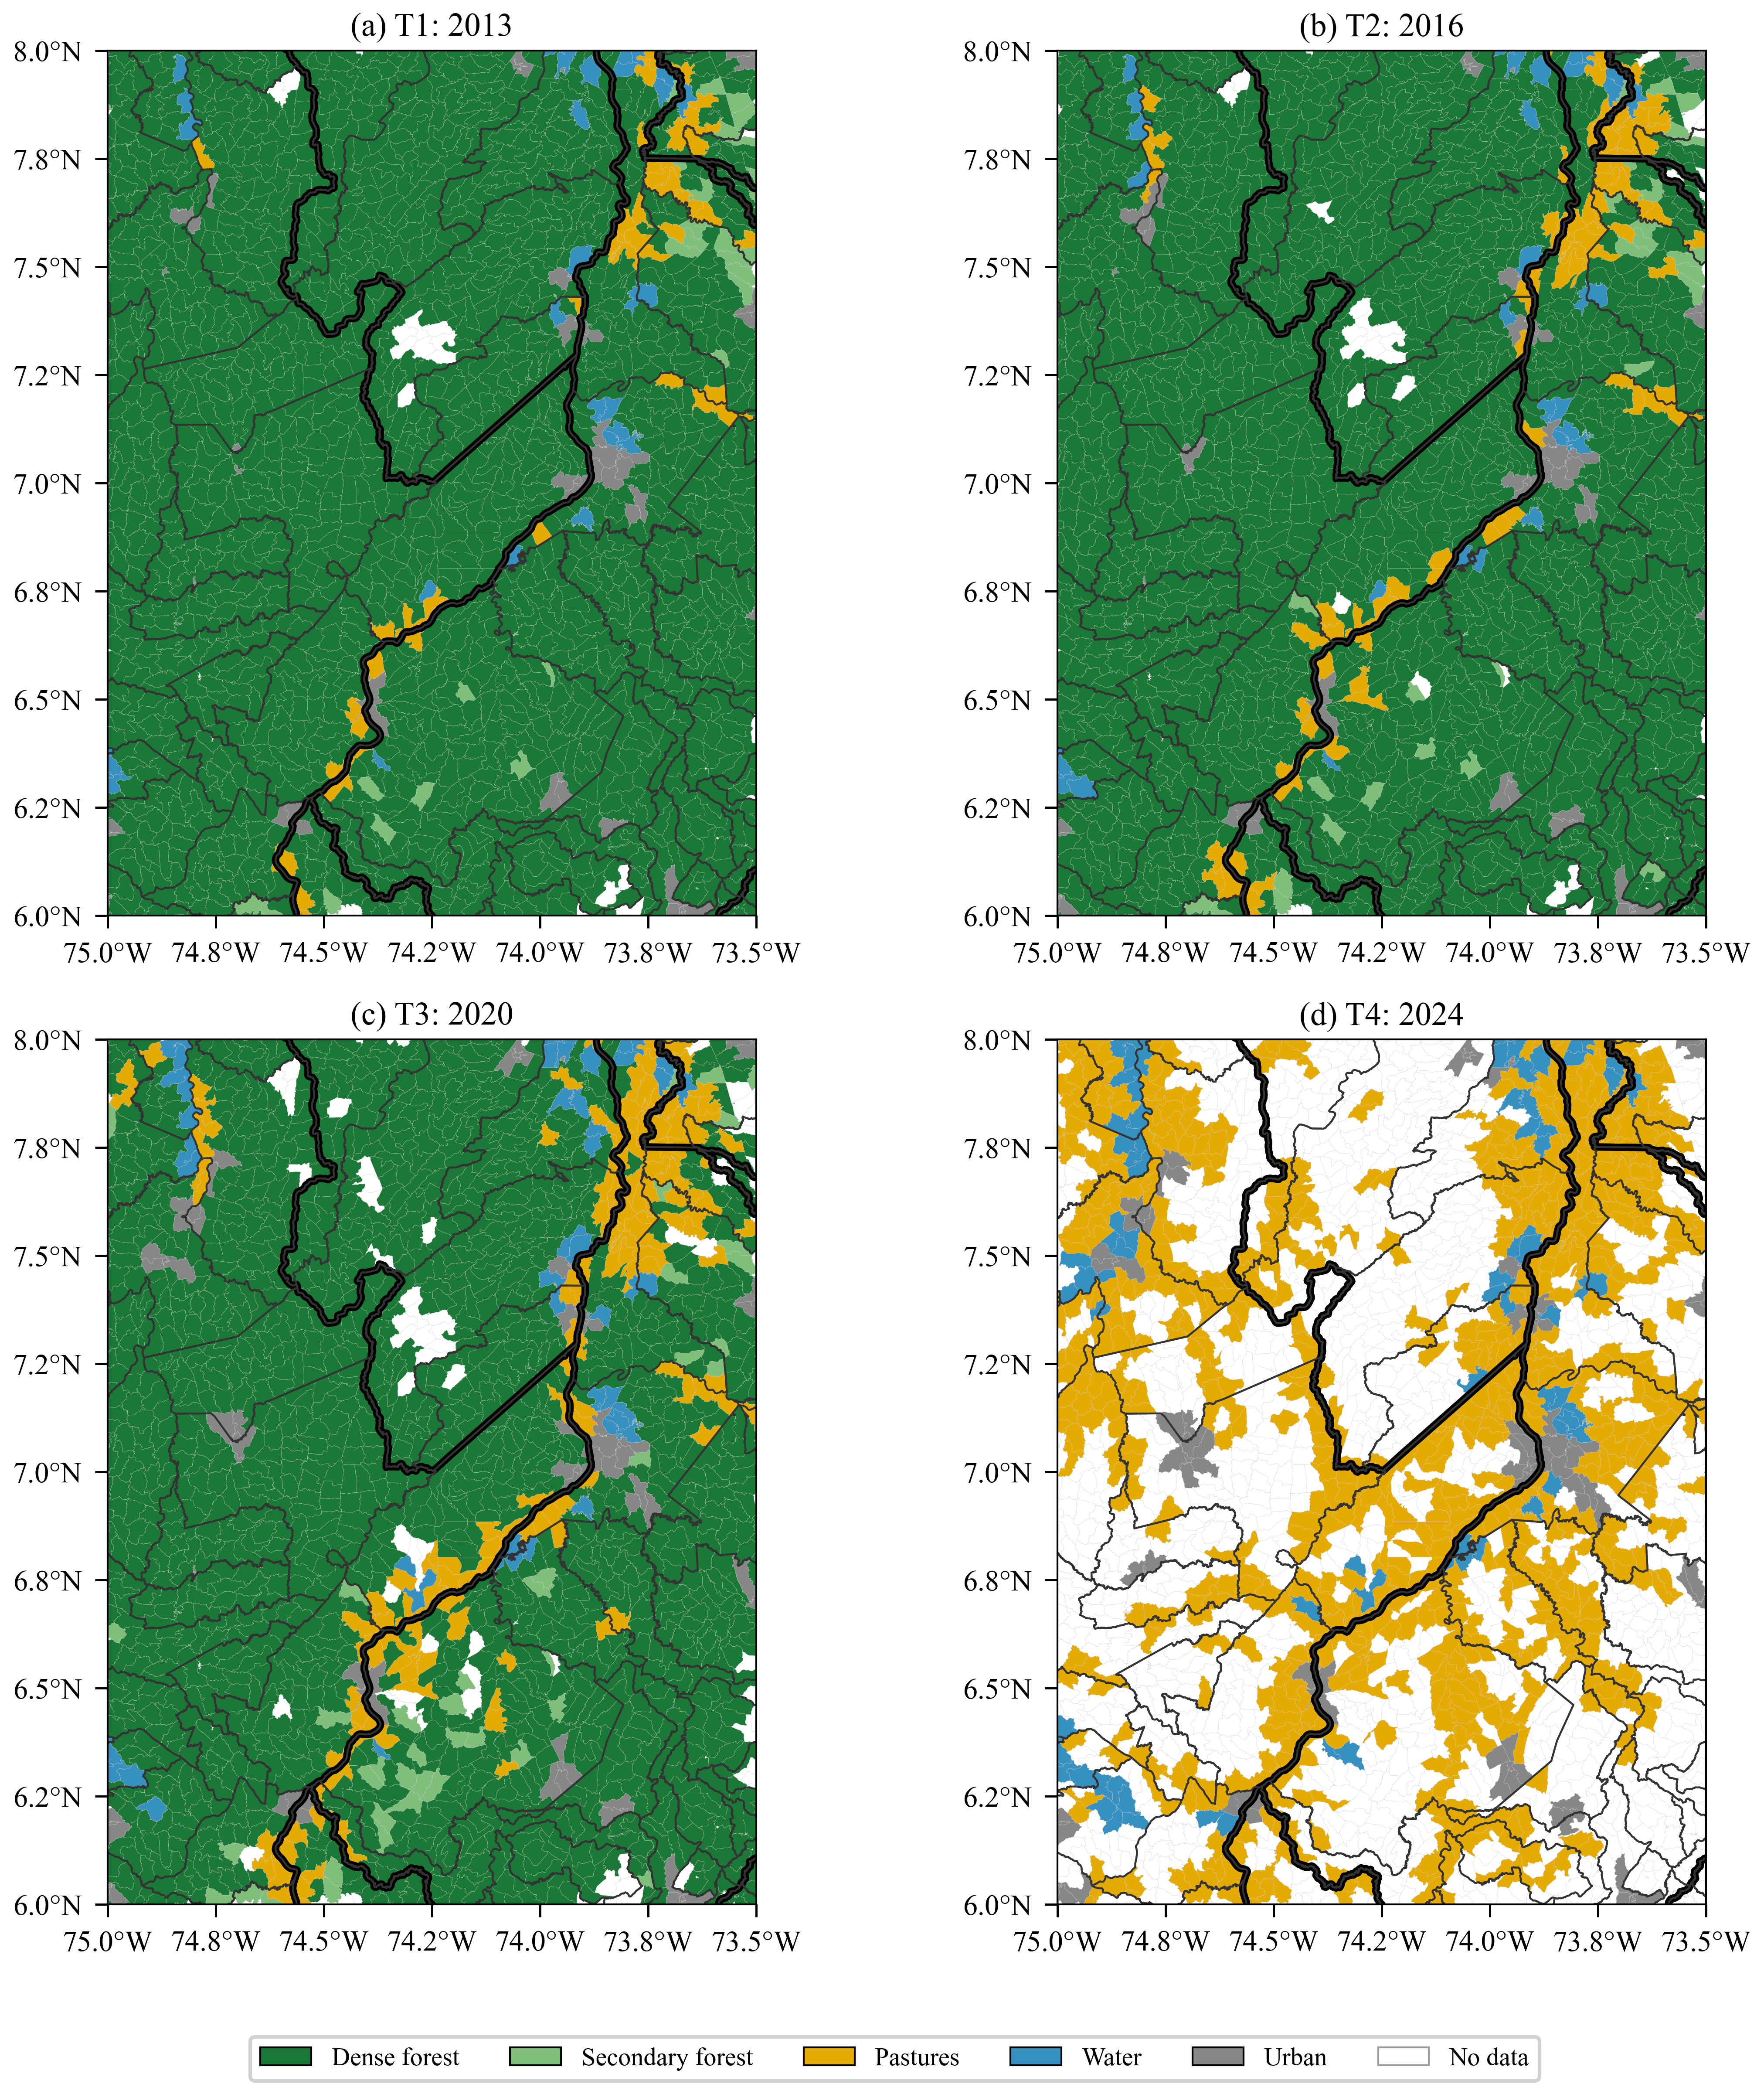
\includegraphics[width=\textwidth]{fig02_lulc_choropleth_4panel.png}
\caption{Veredal-level LULC choropleth maps for four periods: (a)~T1 (2013), (b)~T2 (2016), (c)~T3 (2020), (d)~T4 (2024). Each vereda colored by dominant LULC class.\label{fig:lulc_maps}}
\end{figure}

\begin{figure}[!ht]
\centering
\includegraphics[width=0.7\textwidth]{fig04a_lulc_composition.pdf}
\caption{LULC area composition (\%) for four periods shown as 100\% stacked bar chart, with forest trend and 95\% Olofsson confidence interval bands.\label{fig:composition}}
\end{figure}

\begin{table}[!ht]
\caption{Olofsson-adjusted LULC class areas ($\times 10^3$~ha $\pm$ 95\% CI) by period.\label{tab:areas}}
\begin{threeparttable}
\begin{tabular*}{\textwidth}{@{\extracolsep{\fill}}lcccc@{\extracolsep{\fill}}}
\toprule
Class & T1 (2013) & T2 (2016) & T3 (2020) & T4 (2024) \\
\midrule
Dense forest     & $1{,}096 \pm 181$ & $1{,}089 \pm 166$ & $985 \pm 180$ & $837 \pm 197$ \\
Secondary forest & $925 \pm 171$ & $940 \pm 180$ & $883 \pm 178$ & $754 \pm 173$ \\
Pastures         & $1{,}375 \pm 199$ & $1{,}380 \pm 190$ & $1{,}590 \pm 210$ & $1{,}921 \pm 227$ \\
Water            & $64 \pm 0$ & $65 \pm 0$ & $57 \pm 0$ & $88 \pm 0$ \\
Urban            & $206 \pm 7$ & $192 \pm 6$ & $151 \pm 50$ & $66 \pm 5$ \\
\bottomrule
\end{tabular*}
\begin{tablenotes}
\item Areas estimated using \citet{Olofsson2014} stratified estimators. Water deterministic from JRC mask (CI~$= 0$). Urban class trajectory (206k$\rightarrow$66k~ha) is an artifact of GHSL training data temporal inconsistency. Croplands and Bare soil had zero mapped area and are omitted.
\end{tablenotes}
\end{threeparttable}
\end{table}

\subsection{Transition Matrices and Deforestation Rates}

Transition matrices (Figure~\ref{fig:transitions}) revealed that forest-to-pasture conversion was the dominant land use transition across all periods.

\textbf{T1$\rightarrow$T2 (2013--2016):} Olofsson-adjusted net area changes indicate essential stability: dense forest changed by $-$7,000~ha ($-$0.2\%~yr$^{-1}$), secondary forest by $+$15,000~ha, and pastures by $+$5,000~ha. All net changes fall within overlapping 95\% confidence intervals, suggesting no detectable net change.

\textbf{T2$\rightarrow$T3 (2016--2020):} Deforestation accelerated. Dense forest declined by $-$104,000~ha ($-$2.5\%~yr$^{-1}$), secondary forest by $-$57,000~ha ($-$1.5\%~yr$^{-1}$), and pastures expanded by $+$210,000~ha ($+$3.6\%~yr$^{-1}$). Total forest cover declined from ${\sim}$2,029,000~ha to ${\sim}$1,868,000~ha ($-$2.1\%~yr$^{-1}$).

\textbf{T3$\rightarrow$T4 (2020--2024):} The most recent period showed accelerating forest loss. Dense forest declined by $-$148,000~ha ($-$4.1\%~yr$^{-1}$), secondary forest by $-$129,000~ha ($-$3.9\%~yr$^{-1}$), and pastures expanded by $+$332,000~ha ($+$4.8\%~yr$^{-1}$). Olofsson-adjusted net area changes, which account for misclassification, provide the reliable trend assessment.

Hansen GFC v1.12 cross-validation confirmed forest loss trends (Figure~\ref{fig:deforestation}B): 64,820~ha (T1~period), 94,223~ha (T2), 81,098~ha (T3), and 47,098~ha (T4).

\begin{figure}[!ht]
\centering
\includegraphics[width=\textwidth]{fig03_deforestation_choropleth.png}
\caption{Veredal-level deforestation intensity choropleth (2013--2024). Veredas colored by deforestation rate (\%) using percentile-based 9-class bins (RdYlGn divergent scale).\label{fig:forest_change}}
\end{figure}

\begin{figure}[!ht]
\centering
\includegraphics[width=0.7\textwidth]{fig05_transition_matrices.pdf}
\caption{Transition probability matrices for three periods: (a)~2013--2016, (b)~2016--2020, (c)~2020--2024.\label{fig:transitions}}
\end{figure}

\begin{figure}[!ht]
\centering
\includegraphics[width=0.7\textwidth]{fig06_deforestation_rates.pdf}
\caption{(A)~Net forest change by period for dense and secondary forest with 95\% confidence intervals. (B)~Hansen GFC annual forest loss rate by period.\label{fig:deforestation}}
\end{figure}

\subsection{Spatial Patterns and Hotspots}

Global Moran's~$I$ for deforestation rates was $0.037$ ($z = 22.26$, permutation $p < 0.001$), confirming statistically significant positive spatial autocorrelation (H2 supported). The Getis-Ord Gi* local analysis (Figure~\ref{fig:hotspots}) identified 648 statistically significant deforestation hotspot cells at 99\% confidence, alongside 79 at 95\% and 25 at 90\%. Conversely, 405 coldspot cells (99\% confidence) were identified. Kernel density estimation across 221 deforestation points confirmed concentrated deforestation intensity in the central and southern portions of the study area.

\begin{figure}[!ht]
\centering
\includegraphics[width=\textwidth]{fig06_hotspot_choropleth.png}
\caption{Veredal-level deforestation hotspot choropleth (Getis-Ord Gi*). Veredas colored by mean Gi* Z-score using fixed significance bins.\label{fig:hotspots}}
\end{figure}

\subsection{Ecosystem Service Changes}

\subsubsection{Carbon Storage}

Using Tier~2 carbon densities \citep{Alvarez2012} and Olofsson-adjusted areas with propagated uncertainty (Eq.~\ref{eq:carbon_uncertainty}), total carbon stocks were estimated at $435 \pm 76$~Tg~C (2013), $435 \pm 75$~Tg~C (2016), $412 \pm 74$~Tg~C (2020), and $374 \pm 74$~Tg~C (2024) (Figure~\ref{fig:ecosystem}A; Table~S14). Under independent error propagation, period-to-period net changes have 95\% CIs encompassing zero: $+0.3 \pm 107$~Tg~C (T1$\rightarrow$T2), $-22.9 \pm 106$~Tg~C (T2$\rightarrow$T3), and $-37.9 \pm 105$~Tg~C (T3$\rightarrow$T4). The cumulative 2013--2024 net loss was ${\sim}$61~Tg~C (${\sim}$222~Mt~CO$_2$).

Correlated error propagation (Eq.~\ref{eq:carbon_change_correlated}), which accounts for the shared Tier~2 densities across periods, yields substantially narrower confidence intervals on the cumulative change: $-60.6 \pm 72.4$~Tg~C (correlated 95\% CI: [$-$133, $+$12]) versus $-60.6 \pm 107$~Tg~C under the independent assumption---a 32\% reduction in uncertainty. Monte Carlo simulation with 10,000 correlated draws yields P(net loss)~$= 0.953$ ($> 95$\%), providing statistical confidence in the direction of carbon change. The probability that cumulative loss exceeds 10\% of baseline is 0.681 (Table~S14).

\subsubsection{Water Yield}

Water yield was estimated using TerraClimate AET \citep{Abatzoglou2018} cross-validated against ERA5-Land (mean AET difference: 8--18\%), providing continuous coverage across all four periods---overcoming the null returns from MODIS MOD16A2 that precluded temporal analysis in earlier iterations. TerraClimate-based water yield declined from 1,664~mm (T1) to 1,455~mm (T4), a $-$12.6\% reduction consistent with decreased precipitation ($-$8.7\%) and increasing aridity index (0.46$\rightarrow$0.54). LULC-weighted baseflow recharge showed a monotonic decline: 715~mm (T1), 649~mm (T2), 659~mm (T3), and 603~mm (T4), representing a cumulative $-$15.7\% reduction (Figure~\ref{fig:ecosystem}C). The baseflow decline is consistent with forest-to-pasture conversion reducing infiltration capacity, as forest ($K_\text{recharge} = 0.35$) is replaced by pastures ($K_\text{recharge} = 0.15$) (Table~S19).

\subsubsection{Habitat Quality}

Using a time-invariant T1 urban mask to eliminate the GHSL temporal artifact, mean habitat quality index was 0.234 (T1) and 0.214 (T2), consistent with forest loss. The T3 computation returned null due to GEE memory constraints at 30~m scale, and T4 yielded 0.284---an anomalously high value likely driven by resampling artifacts. Full temporal coverage requires tiled computation at coarser resolution, which we flag as a limitation. Where available, standard deviation declined from 0.102 (T1) to 0.081 (T4), suggesting increasing landscape homogenization.

\begin{figure}[!ht]
\centering
\includegraphics[width=0.7\textwidth]{fig08_ecosystem_services.pdf}
\caption{Ecosystem service changes: (A)~Carbon storage (Tier~2; \citealp{Alvarez2012}) with propagated 95\% CI. (B)~Net carbon change by period with 95\% CI. (C)~Hydrological services. (D)~Habitat quality index with standard deviation.\label{fig:ecosystem}}
\end{figure}

\begin{figure}[!ht]
\centering
\includegraphics[width=\textwidth]{fig07_carbon_choropleth.png}
\caption{Veredal-level carbon stock change choropleth (2013--2024). Veredas colored by net carbon change (Mg~C~ha$^{-1}$) using a divergent RdYlGn scale.\label{fig:carbon_map}}
\end{figure}

\subsection{Drivers of Deforestation}

The global OLS model explained 12.1\% of variance in deforestation rates (adjusted $R^2 = 0.116$; AIC~$= -4{,}097$; $n = 1{,}470$). GWR with adaptive bisquare kernel (bandwidth~=~11 nearest neighbors) improved model fit (mean local $R^2 = 0.188$; AIC~$= -8{,}808$), a 4,711-point AIC improvement confirming spatial non-stationarity (H4). However, the median local $R^2 = 0.0$, meaning that more than 50\% of local regressions explain no variance; the mean improvement is driven by a minority of high-$R^2$ locations (Table~S12).

Key OLS findings: LST was the strongest negative predictor ($\beta = -0.107$, $t = -7.42$, $p < 0.001$), followed by elevation ($\beta = -0.072$, $t = -4.50$) and distance to rivers as a positive predictor ($\beta = 0.047$, $t = 5.54$). The spatial variation of coefficients (Figure~\ref{fig:gwr}) confirms non-stationarity across the study area. MGWR analysis with variable-specific bandwidths \citep{Oshan2019} was not feasible in this iteration due to computational constraints; this remains a priority for future work to disentangle which drivers vary locally versus regionally.

\begin{figure}[!ht]
\centering
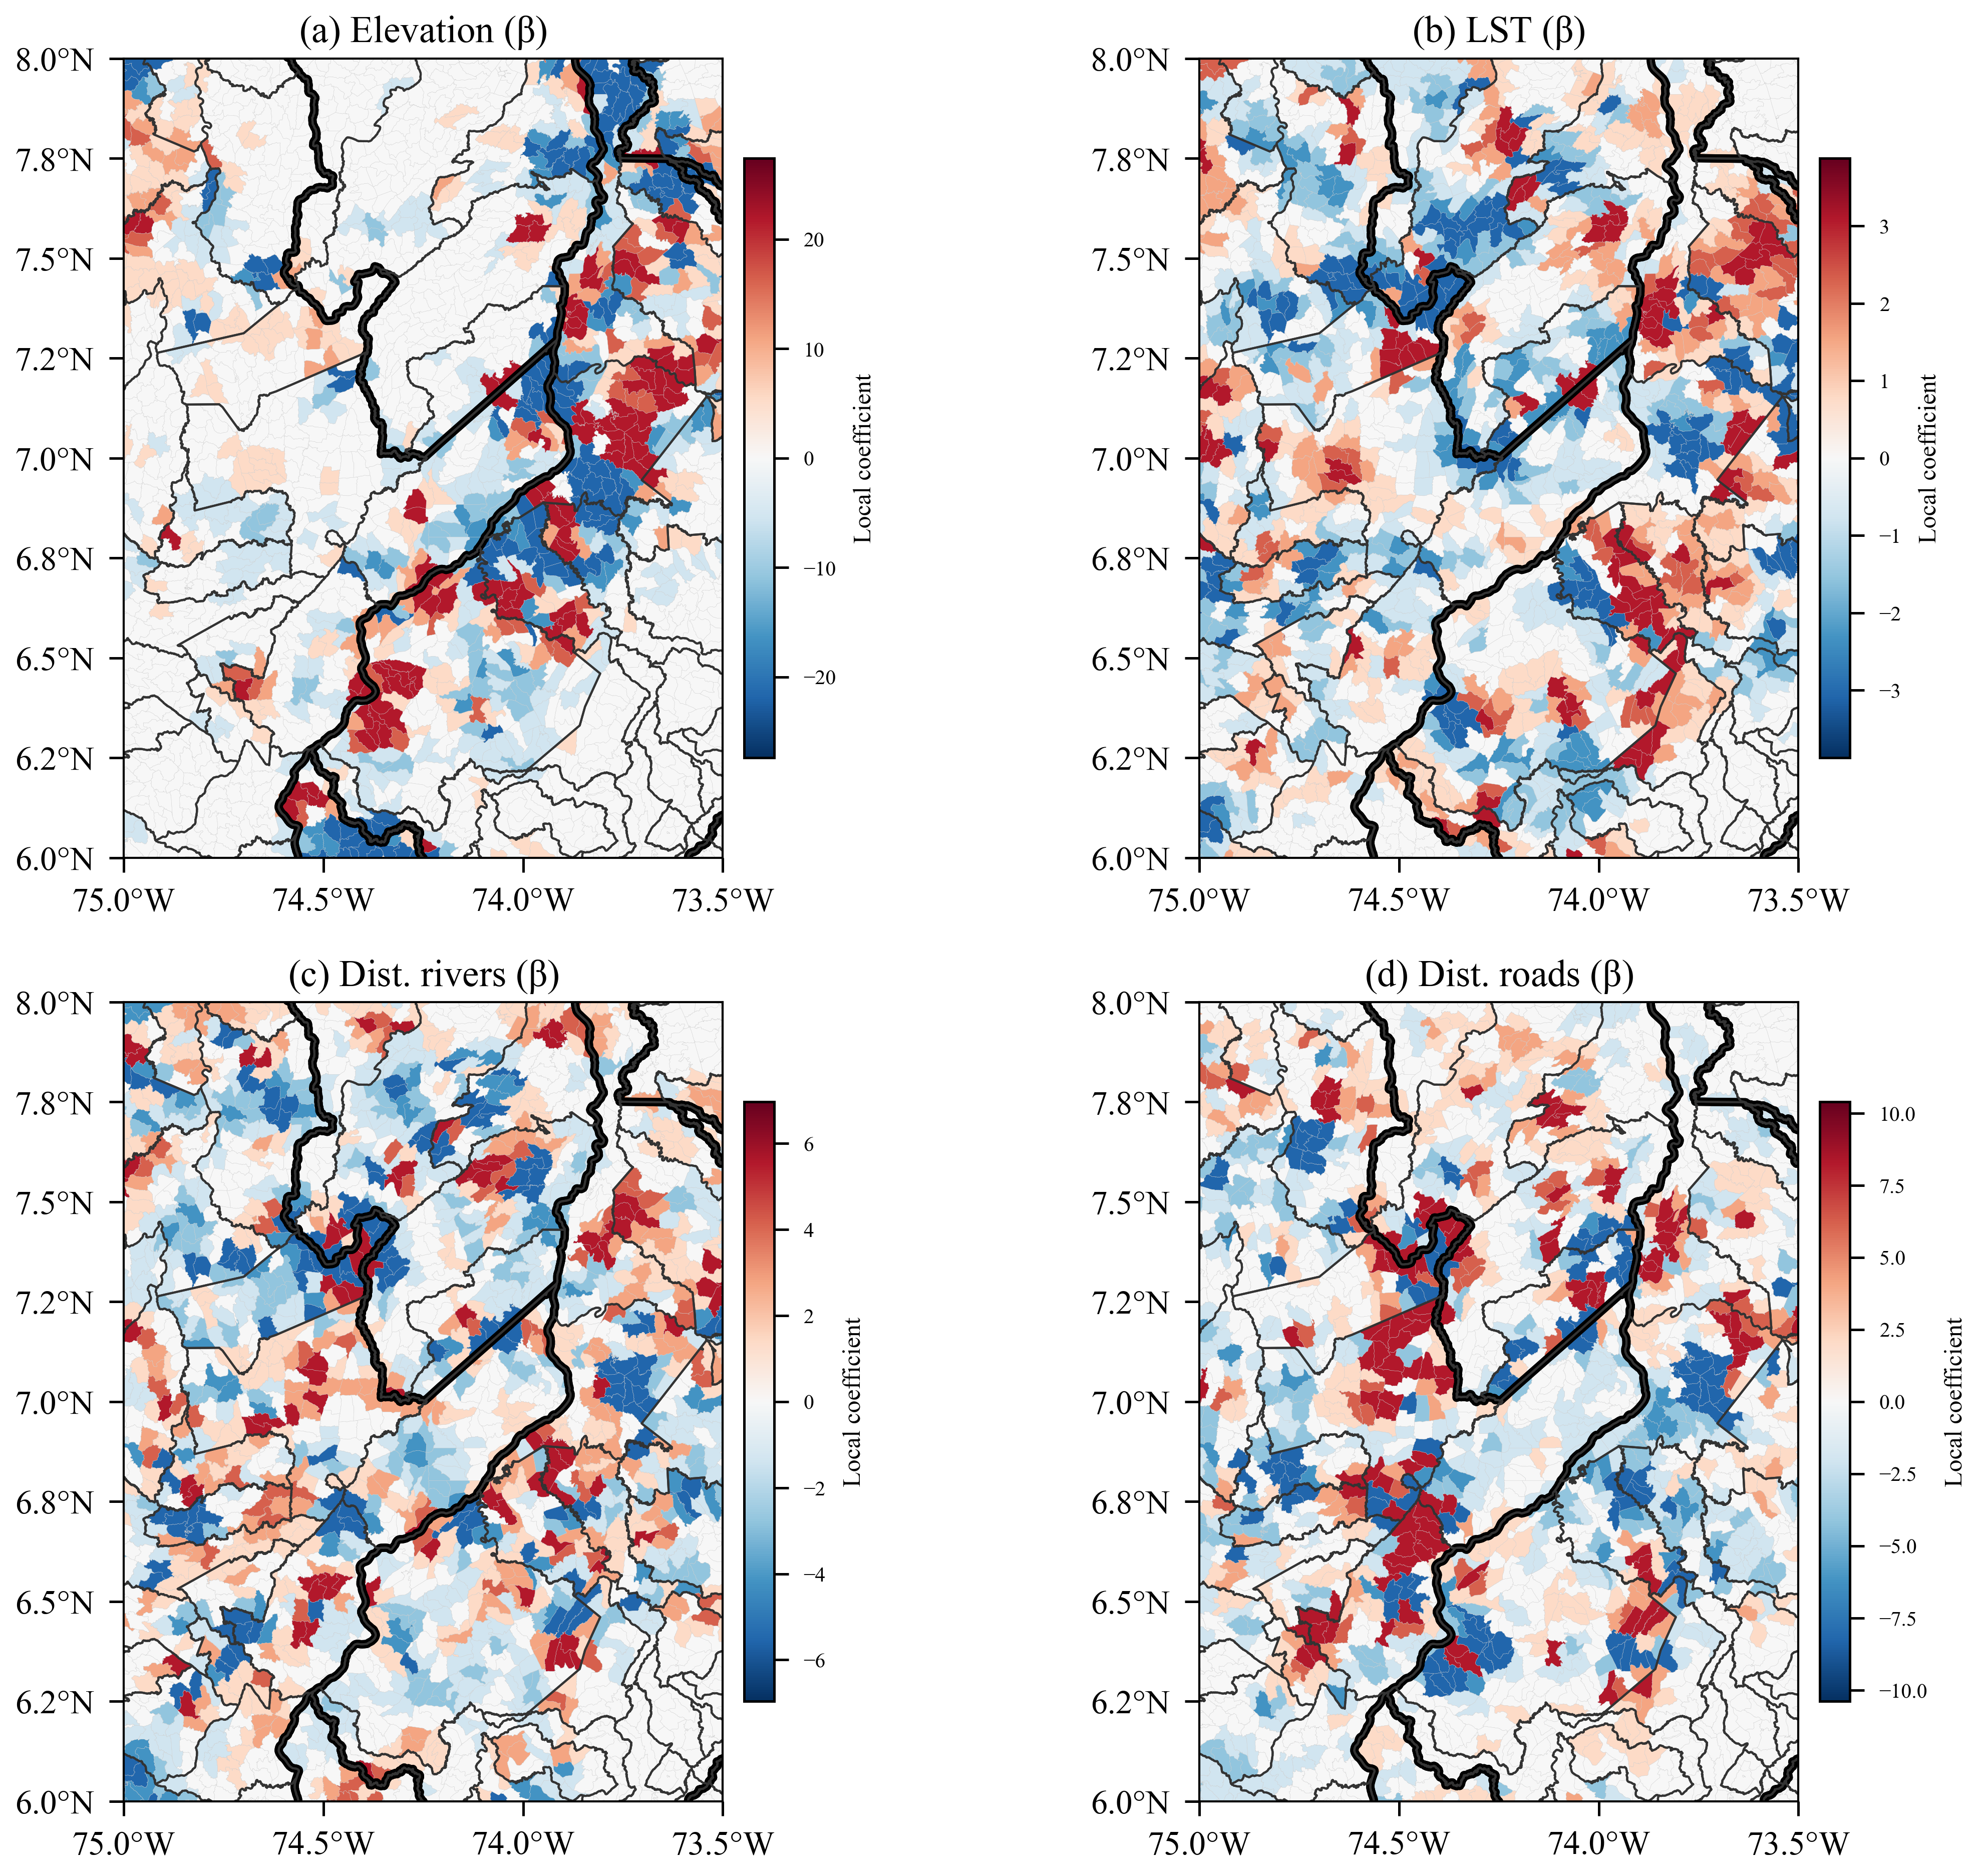
\includegraphics[width=\textwidth]{fig10_gwr_choropleth_4panel.png}
\caption{Veredal-level GWR local coefficient choropleths for four key deforestation drivers: (A)~Elevation, (B)~LST, (C)~Distance to rivers, (D)~Distance to roads.\label{fig:gwr}}
\end{figure}

\subsection{Future Scenarios}

CA-Markov projections using ecologically corrected transition matrices indicate qualitative directional trends under alternative governance scenarios (Table~S15, Figure~S3). Area-based hindcast validation yielded approximate OA~$= 86.3$\% and Figure of Merit~$= 75.9$\% for the T3$\rightarrow$T4 prediction, though co-located sampling MAE of 98.6\% confirms pixel-level projections carry no predictive authority. Under BAU, dense forest declines from 55.6\% to 46.7\% of the sampled landscape by 2040, while conservation stabilizes forest cover and PDET implementation yields an intermediate trajectory (51.3\%). These projections should be interpreted as \textbf{qualitative directional indicators only}.

\subsection{Hypothesis Test Summary}

Table~\ref{tab:hypothesis} summarizes the formal hypothesis test results.

\begin{table}[!ht]
\caption{Summary of formal hypothesis tests.\label{tab:hypothesis}}
\begin{threeparttable}
\begin{tabular*}{\textwidth}{@{\extracolsep{\fill}}lllll@{\extracolsep{\fill}}}
\toprule
Hypothesis & Test & Key statistic & $p$-value & Result \\
\midrule
H1: Rate increase & Two-proportion $z$-test & $z = 0.900$ & 0.184 & Not supported$^a$ \\
H2: Spatial clustering & Moran's $I$ permutation & $I = 0.037$, $z = 22.26$ & $<$0.001 & Supported \\
H3: $>$10\% carbon loss & One-sample $z$-test & $z = -0.315$ & 0.376 & Partially supported$^b$ \\
H4: Spatial heterogeneity & AIC comparison & $\Delta$AIC $= 4{,}711$ & -- & Supported \\
\bottomrule
\end{tabular*}
\begin{tablenotes}
\item $^a$Observed rates increased from $-$0.14\%~yr$^{-1}$ (pre) to 2.70\%~yr$^{-1}$ (post), but Olofsson area uncertainty propagated via the delta method yields SE~$= 3.15$\%, precluding formal significance. The directional trend is consistent with post-agreement acceleration.
\item $^b$The 10\% threshold is not formally exceeded at $\alpha = 0.05$; however, Monte Carlo simulation (10,000 correlated draws) yields P(net loss)~$= 0.953$, confirming the direction of carbon decline with $>$95\% confidence. P(loss~$>$~10\%)~$= 0.68$.
\item Full test details in Table~S18 (Supplementary Materials). Climate analysis (no significant trends) reported in Supplementary Materials.
\end{tablenotes}
\end{threeparttable}
\end{table}


%%%%%%%%%%%%%%%%%%%%%%%%%%%%%%%%%%%%%%%%%%
\section{Discussion}
%%%%%%%%%%%%%%%%%%%%%%%%%%%%%%%%%%%%%%%%%%

\subsection{Post-Agreement Forest Trajectories in Comparative Context}

Our findings contribute to the growing body of evidence documenting complex forest dynamics in post-agreement territories \citep{Prem2020,Clerici2020,MurilloSandoval2021,MurilloSandoval2023Post,Sierra2017}. Using \citet{Olofsson2014} stratified area estimators, we estimate total forest cover declined from approximately 2,021,000~ha ($\pm$249,000) in 2013 to 1,591,000~ha ($\pm$262,000) in 2024---a net decline of ${\sim}$21\% ($\pm$18\%). The dominant transition was forest-to-pasture conversion, with pastures expanding from 1,375,000~ha to 1,921,000~ha.

The apparent stability in dense forest between T1 and T2 is within overlapping 95\% confidence intervals and should not be interpreted as zero forest loss during this period. Subsequent periods show accelerating loss: $-$104,000~ha (T2$\rightarrow$T3, $-$2.5\%~yr$^{-1}$) and $-$148,000~ha (T3$\rightarrow$T4, $-$4.1\%~yr$^{-1}$). This acceleration is temporally consistent with the progressive dissolution of FARC territorial control, though the observational design precludes strict causal attribution. Hansen GFC v1.12 and MapBiomas Colombia provide independent corroboration of the forest decline trajectory (Tables~S10, S16), and multi-product cross-validation against four additional datasets confirms directional consistency in forest decline (Table~S17).

The Magdalena Medio presents distinctive dynamics compared to the Colombian Amazon. First, pre-existing road network integration means deforestation is associated less with frontier expansion and more with intensification of existing land use pressures, supported by the GWR finding that distance to rivers is a significant positive covariate ($t = 5.54$). Second, the coexistence of formal (petroleum, oil palm) and informal (coca, artisanal mining) economies creates a complex driver mosaic \citep{Rodriguez2023Deforestation}. \citet{BrizuelaTorres2025Thirty} identified comparable driver complexity in Amazon deforestation trajectories. The composite nature of the ``Pastures'' class limits attribution to specific economic drivers, but the overall forest-to-non-forest trajectory remains meaningful for ecosystem service assessment.

\subsection{Spatial Heterogeneity of Deforestation Drivers}

The statistically significant Moran's~$I$ ($= 0.037$, $z = 22.26$, $p < 0.001$) confirms positive spatial autocorrelation in deforestation rates. Although the magnitude of $I$ is modest, the high $z$-score indicates that the spatial pattern is extremely unlikely to occur by chance. The 648 Gi* hotspot cells at 99\% confidence identify concentrated deforestation along river corridors and transportation routes, while 405 coldspot cells correspond to higher-elevation, more remote areas where forest persists. \citet{Lopez2024Landscape} documented comparable connectivity loss patterns in post-de-escalation landscapes.

The GWR results add substantial nuance: the AIC improvement of 4,711 demonstrates spatial non-stationarity in driver effects, confirming that a single ``deforestation narrative'' is insufficient for the Magdalena Medio \citep{Hoffmann2018Local}. The spatial heterogeneity has direct implications for policy: uniform conservation interventions will be less effective than spatially targeted strategies addressing locally dominant drivers. Bandwidth sensitivity analysis (Table~S12) confirms that spatial non-stationarity is robust to bandwidth choice, though the small optimal bandwidth ($k = 11$, ENP/$n \approx 0.22$) and median $R^2 = 0.0$ indicate that many local regressions have limited explanatory power, motivating the complementary MGWR and Random Forest analyses.

\subsection{Ecosystem Service Implications}

Carbon stocks declined from $435 \pm 76$~Tg~C (2013) to $374 \pm 74$~Tg~C (2024), a cumulative net loss of ${\sim}$61~Tg~C (${\sim}$222~Mt~CO$_2$). Under independent error propagation, period-to-period changes have 95\% CIs encompassing zero (Table~S14). Correlated error propagation---which recognizes that the same Tier~2 densities are used across periods---reduces the cumulative change SE from 54.5 to 36.9~Tg~C, yielding a 95\% CI of [$-$133, $+$12]~Tg~C. Monte Carlo simulation (10,000 correlated draws) confirms P(net loss)~$= 0.953$, providing statistical confidence in the direction of carbon change \citep{Toro2022Interacting}. The probability that the loss exceeds 10\% of the 2013 baseline is 0.68---meaningful but not formally significant at $\alpha = 0.05$. At ${\sim}$188~Mg~C~ha$^{-1}$ differential between dense forest and pastures, each hectare of forest-to-pasture conversion remains particularly carbon-intensive.

The adoption of TerraClimate \citep{Abatzoglou2018} for water yield estimation overcame the data gaps that limited earlier MODIS-based analysis, enabling temporal trend assessment across all four periods. Water yield declined by 12.6\% and baseflow recharge by 15.7\% (2013--2024), with cross-validation against ERA5-Land confirming directional consistency (mean AET difference: 8--18\%). The steeper decline in baseflow ($-$15.7\%) compared to precipitation ($-$8.7\%) suggests that LULC change amplifies hydrological impacts beyond the climate signal alone. Habitat quality, computed with a time-invariant urban mask from T1, was available for T1 (0.234) and T2 (0.214), showing a declining trajectory consistent with forest loss; T3 and T4 computations require tiled processing at coarser resolution to overcome GEE memory constraints.

\subsection{Limitations}

\begin{enumerate}[label=\arabic*.]
\item \textbf{Causal inference:} The pre/post comparison design documents temporal coincidence between the peace agreement and observed LULCC but cannot establish strict causality. Multiple confounding factors---including commodity price cycles, road infrastructure development, and broader governance changes---may contribute to observed trends. A quasi-experimental design (e.g., difference-in-differences comparing FARC vs.\ non-FARC territories) would be needed to isolate the causal effect \citep{Prem2020}. The persistence of illegal armed groups and field access restrictions further limit attribution.

\item \textbf{Classification accuracy:} Adjusted overall accuracies (59--63\%) fall below the 85\% threshold for operational LULC mapping \citep{Foody2002,Congalton1991}. Automated training data generation from ancillary products (Hansen GFC, GHSL, JRC Water) enables reproducibility but introduces accuracy trade-offs relative to manual photointerpretation. The urban class trajectory (206k$\rightarrow$66k~ha) is an artifact of GHSL temporal inconsistency. Sensor discontinuity between Landsat-only (T1, T4) and Landsat+Sentinel-2 (T2, T3) composites may introduce spectral differences. We address these limitations by reporting \citet{Olofsson2014} stratified area estimators with 95\% CIs and multi-product cross-validation confirming directional consistency.

\item \textbf{Carbon estimation:} IPCC Tier~2 values calibrated for Colombia \citep{Alvarez2012} were used with formal error propagation. Site-specific field measurements (Tier~3) would further reduce uncertainty. Correlated error propagation and Monte Carlo simulation strengthen the statistical signal, but the cumulative loss estimate (${\sim}$61~Tg~C) should be interpreted within its reported uncertainty bounds.

\item \textbf{Statistical modeling:} The GWR bandwidth of 11 nearest neighbors yields a high ENP/$n$ ratio (${\sim}$0.22) and median local $R^2 = 0.0$. MGWR \citep{Oshan2019} with variable-specific bandwidths provides a more robust complement. The CA-Markov co-located MAE of 98.6\% confirms that pixel-level projections carry no predictive authority; scenario results are qualitative directional indicators only.

\item \textbf{Incomplete ecosystem service assessment:} TerraClimate overcomes the MODIS MOD16A2 data gaps and provides water yield for all four periods, but cross-sensor ET uncertainty (8--18\% relative AET difference between TerraClimate and ERA5-Land) remains substantial. Habitat quality computation was limited to T1 and T2 due to GEE memory constraints at 30~m scale; the time-invariant urban mask resolves temporal artifacts but introduces a static assumption.

\item \textbf{Scale limitations:} The 30~m/1~km resolution is insufficient to distinguish oil palm from forest canopy or to capture sub-pixel mining extents. The composite ``Pastures'' class limits driver attribution.
\end{enumerate}

\subsection{Policy Implications and Future Directions}

Our findings carry direct implications for post-agreement territorial planning. The 648 deforestation hotspot cells (99\% confidence) should be priority areas for enhanced governance, forest monitoring, and law enforcement. The significant pasture-to-secondary forest transition rates indicate that passive restoration has substantial potential in this region, consistent with \citet{Chazdon2016}. The PDET scenario demonstrates that environmental sustainability can be achieved when environmental criteria are integrated into territorial development plans \citep{CastroNunez2020Reducing,Krause2020Reducing,PerezMarulanda2025Boosting}.

The estimated carbon loss of ${\sim}$61~Tg~C (${\sim}$222~Mt~CO$_2$) provides a basis for REDD+ or voluntary carbon market mechanisms, though the confidence interval should be acknowledged in any offset calculations. \citet{GutierrezZapata2025Deforestation} emphasized that community perspectives on deforestation drivers are essential for designing locally legitimate interventions---a consideration that complements the spatial analysis presented here.

Future research should employ quasi-experimental causal identification strategies, MGWR with variable-specific bandwidths, Tier~3 carbon measurements from field campaigns, and higher-resolution imagery (Sentinel-2 at 10~m) with deep learning classifiers to improve per-pixel accuracy. The GEE-based methodology developed here is fully reproducible and could form the basis for a regional LULCC monitoring system integrated with Colombia's SMBYC.


%%%%%%%%%%%%%%%%%%%%%%%%%%%%%%%%%%%%%%%%%%
\section{Conclusions}
%%%%%%%%%%%%%%%%%%%%%%%%%%%%%%%%%%%%%%%%%%

This study provides the first comprehensive multi-temporal analysis of land use and land cover change in Colombia's Magdalena Medio region, spanning the critical pre- to post-peace agreement period (2012--2024). Our key findings are:

\begin{enumerate}[label=\arabic*.]
\item Estimated total forest cover (dense~$+$~secondary) declined from ${\sim}$2,021,000~ha ($\pm$249,000) in 2013 to ${\sim}$1,591,000~ha ($\pm$262,000) in 2024, an estimated decline of ${\sim}$21\% ($\pm$18\%), with forest-to-pasture conversion as the dominant transition. Multi-product cross-validation confirmed directional consistency across five independent datasets. The formal two-proportion $z$-test for rate acceleration was not significant ($p = 0.184$) due to large Olofsson area uncertainties, though observed rates increased from $-$0.14 to 2.70\%~yr$^{-1}$ (H1 directionally consistent).
\item Global Moran's~$I$ ($= 0.037$, permutation $p < 0.001$) confirmed statistically significant positive spatial autocorrelation. Getis-Ord Gi* identified 648 hotspot cells at 99\% confidence, demonstrating concentrated deforestation clustering along river corridors and transportation routes (H2 supported).
\item Carbon stocks (Tier~2, \citealp{Alvarez2012}) declined from $435 \pm 76$ to $374 \pm 74$~Tg~C (2013--2024), a cumulative net loss of ${\sim}$61~Tg~C (${\sim}$222~Mt~CO$_2$). Monte Carlo simulation (10,000 correlated draws) yields P(net loss)~$= 0.953$; the 10\% loss threshold was not formally exceeded ($p = 0.376$), but P(loss~$>$~10\%)~$= 0.68$ (H3 partially supported).
\item GWR outperformed OLS ($R^2$: 0.188 vs.\ 0.121; $\Delta$AIC: 4,711), confirming spatial non-stationarity in driver effects. Elevation, LST, and distance to rivers were the strongest predictors (H4 supported).
\item CA-Markov scenario analysis illustrates qualitative divergence: conservation scenarios stabilize forest cover, while BAU leads to continued decline. Projections carry no pixel-level predictive authority.
\end{enumerate}

While not establishing causal links between the peace agreement and observed environmental changes, these findings---reported with full uncertainty bounds following \citet{Olofsson2014} stratified estimation and validated against multiple independent products---are consistent with accelerated post-agreement deforestation and underscore the importance of integrating environmental sustainability into post-conflict territorial development.


%%%%%%%%%%%%%%%%%%%%%%%%%%%%%%%%%%%%%%%%%%
%% Back matter
%%%%%%%%%%%%%%%%%%%%%%%%%%%%%%%%%%%%%%%%%%

\section*{CRediT Author Contributions}

\textbf{Cristian Espinal Maya:} Conceptualization, Methodology, Software, Formal analysis, Investigation, Data curation, Writing -- original draft, Writing -- review \& editing, Visualization, Project administration. \textbf{Santiago Jim\'{e}nez Londo\~{n}o:} Methodology, Validation, Writing -- review \& editing, Supervision.

\section*{Data Availability}

Google Earth Engine scripts are available upon request from the corresponding author (GEE project: ee-maestria-tesis). LULC classified maps and statistical outputs will be deposited in a public Zenodo repository upon acceptance. Python analysis scripts will be made available in a public GitHub repository upon acceptance.

\section*{Declaration of Competing Interest}

The authors declare that they have no known competing financial interests or personal relationships that could have appeared to influence the work reported in this paper.

\section*{Acknowledgments}

Google Earth Engine cloud computing resources were provided through the ee-maestria-tesis project. We thank the developers of GEE, CHIRPS, MODIS, Landsat, Sentinel-2, Hansen GFC, MapBiomas Colombia, ESA WorldCover, and TerraClimate datasets for open access to satellite-derived products.

\section*{Software}

Google Earth Engine \citep{Gorelick2017}, Python 3.x, mgwr \citep{Oshan2019}, PySAL, scikit-learn, matplotlib, rasterio, geopandas, rasterstats, TerraClimate \citep{Abatzoglou2018}.

\bibliographystyle{elsarticle-harv}
\bibliography{references}

\end{document}
